\documentclass[dvipsnames,a4paper]{scrartcl}

\usepackage{import}

\import{./}{lib.tex}

\begin{document}

% HP tracker
\begin{tikzpicture}[overlay,remember picture]
\begin{scope}[shift=(current page.center)]
    % Define the grid size
    \def\rows{16}
    \def\cols{10}
    \def\cellsize{16.68mm}
    
    % Calculate the total width and height of the grid
    \def\gridwidth{\cols*\cellsize}
    \def\gridheight{\rows*\cellsize}
    
    % Draw the grid
    \draw[step=\cellsize] (-0.5*\gridwidth, -0.5*\gridheight) grid (0.5*\gridwidth, 0.5*\gridheight);
    
    \foreach \y in {15,...,0}
        \foreach \x in {1,...,10}
            \pgfmathsetmacro\z{int(\x+(10*\y))}
            \node at (-0.5*\gridwidth+\x*\cellsize-\cellsize/2,-0.5*\gridheight+\y*\cellsize+\cellsize/2) {\z};

\end{scope}
\end{tikzpicture}

\end{document}
